\chapter{\IfLanguageName{dutch}{Stand van zaken}{State of the art}}%
\label{ch:stand-van-zaken}

% Tip: Begin elk hoofdstuk met een paragraaf inleiding die beschrijft hoe
% dit hoofdstuk past binnen het geheel van de bachelorproef. Geef in het
% bijzonder aan wat de link is met het vorige en volgende hoofdstuk.

% Pas na deze inleidende paragraaf komt de eerste sectiehoofding.

Dit onderzoek zal zich dus focussen op wat de voor- en nadelen zijn van het implementeren van 3D elementen in e-commerce. Maar alvorens hieraan te beginnen zal eerst een kijk genomen worden naar wat React en Node.js zijn omdat deze een integraal deel uitmaken voor het opbouwen van de POC's. Nadien zal een grondig onderzoek gedaan worden naar Three.js en welke mogelijkheden dit framework aan te bieden heeft.

\section{React}

React is een open-source front-end JavaScript bibliotheek voor het bouwen van UI componenten. Het wordt onderhouden door Facebook en een gemeenschap van individuele developers en bedrijven \autocite{Bhupati2021}. Tegenwoordig behoort React tot een van de meest gebruikte frameworks voor developers om web applicaties te maken. Voor degenen die nog niet bekend zijn met React, zal er een korte introductie gegeven worden. Voor anderen dient dit hoofdstuk als een opfrissing over de belangrijkste kenmerken van React.

\subsection{Componenten}
De sterkte van React stemt af van de focus op individuele componenten. Deze componenten kunnen developers gemakkelijk hergebruiken om web applicaties te ontwikkelen. Componenten zijn losstaande en herbruikbare stukjes code. Ze vervullen dezelfde functie als JavaScript-functies maar werken geïsoleerd en geven HTML code terug. Componenten komen voor in twee vormen, klasse componenten en functie componenten , de best-practice is momenteel om de functievorm te gebruiken \autocite{W3Schools2023}. Deze componenten kunnen ook genest worden, zo kunnen we componenten maken die gebruikt worden in meerdere web applicaties omdat ze los staan van de gehele applicatie.

\subsection{Props}
Componenten zijn dus een krachtige tool, maar wat als je een component nodig hebt waarbij bepaalde variabelen kunnen veranderen, zoals een afbeelding of een stuk tekst? Hier komen props in het verhaal terecht. Net zoals je bij een afbeelding de 'src' meegeeft kan je bij React-componenten ook aangepaste props meegeven. Dit kan men doen door in de component-tag een waarde toe te kennen aan de prop en deze vervolgens te destructureren in de parameters van de component \autocite{NextJS2023}. Op deze manier kunnen developers op een eenvoudige manier gegevens tussen componenten uitwisselen.

\subsection{Hooks}
Het derde fundamentele concept van React zijn 'hooks'. Hooks bieden de mogelijkheid om extra logica toe te voegen aan je componenten, gebaseerd op een 'state'. Een state is een stuk informatie in de UI dat gedurende de tijd kan veranderen, meestal als gevolg van een interactie van de gebruiker \autocite{NextJS2023}. Stel dat een gebruiker bijvoorbeeld de optie heeft om op een 'Toon Meer' knop te klikken. Hiervoor kan perfect de \texttt{useState(false)} state gebruikt worden. Als de gebruiker op de knop klikt, kunnen we de state wijzigen naar \texttt{true}, wat zal resulteren in het tonen van meer items.

\section{Node.js}

Node.js is een open-source, cross-platform JavaScript runtime omgeving gebouwd op de V8 JavaScript engine van Chrome. Het werd voor het eerst uitgebracht in 2009 door Ryan Dahl en is sindsdien een van de meest populaire frameworks voor het bouwen van schaalbare, high-performance server-side applicaties. \autocite{Sufiyan2023} In dit hoofdstuk zal een korte samenvatting gegeven worden over Node.js.

\subsection{Niet-Blokkerend Asynchroon I/O}

Niet-blokkerende code verwijst naar code die de uitvoering niet vertraagt. Het grote voordeel van niet-blokkerende, asynchrone bewerkingen is dat je hiermee het gebruik van zowel de CPU als het geheugen kunt maximaliseren \autocite{Sarkar2018}.

Node.js probeert dus optimaal gebruik te maken van de CPU a.d.h.v. asynchrone bewerkingen. Dit zorgt ervoor dat het een goede optie is voor schaalbare toepassingen.

\newpage

\section{Three.js}

De lessen van Three.js Journey worden opgedeeld in 7 hoofdstukken met een totaal van 54 lessen. De hoofdstukken zijn:
\begin{itemize}
	\item[1] Basics
	\item[2] Classic techniques
	\item[3] Advanced techniques
	\item[4] Shaders
	\item[5] Extra
	\item[6] Portal Scene
	\item[7] React Three Fiber
\end{itemize}
Voor dit onderzoek zijn alleen hoofdstuk één, twee, drie en zeven van toepassing.

\subsection{Basis}

In volgend hoofdstuk worden de basiscomponenten van Three.js overlopen.

\subsubsection{WebGL}

WebGL is een Javascript API die driehoeken kan tekenen op een canvas met uiterste efficiëntie. Wanneer een gebruiker een website opent met WebGL zal deze API gebruikmaken van de GPU van de gebruiker. De mogelijkheden van WebGL rijken ook verder dan het tekenen van driehoeken zoals 2D ervaringen maar hier zal de focus voornamelijk gelegd worden op 3D ervaringen \autocite{Simon2023}.

Stel dat we een 3D model willen tekenen dat bestaat uit 1000 driehoeken. Elke driehoek bestaat uiteraard 3 punten dus d.w.z. 3000 punten in het totaal. De kracht van de GPU is dat het parallelle calculaties kan uitvoeren en zal zo dus de posities van deze punten in één keer uitvoeren \autocite{Simon2023}.

Nu de posities van de punten bekend zijn moet de GPU de punten plaatsen en elke pixel tekenen. De instructies die dit mogelijk maken noemen we shaders, en deze kunnen snel complex worden. Als er bijvoorbeeld een transformatie gebeurd van het model of de camera maakt een beweging dan moet er data worden doorgegeven aan de shaders en hiervoor gebruiken we matrices. Deze transformatie of camera beweging zal ook veranderingen aanbrengen in de kleur van elke pixel. Driehoeken die zich naar het licht toe positioneren zullen een lichtere kleur krijgen dan degene die dat niet doen \autocite{Simon2023}.

WebGL communiceert dus rechtstreeks met de GPU en dit geeft de developer de mogelijkheid om een volledige controle uit te oefenen over de modellen, camera, licht, perspectief en nog veel meer. Maar hiervoor moet alles wel handmatig geschreven worden, zo kan er voor het tekenen van één driehoek al een 100-tal lijnen code nodig zijn. Dit is dus wat WebGL zo complex maakt.

\subsubsection{Three.js, de gulden middenweg}

Omdat WebGL zo complex is er een oplossing nodig zodat developers geen duizenden lijnen code moeten schrijven iedere keer ze een 3D model willen tekenen. Hiervoor heeft Ricardo Cabello aka Mr.doob Three.js gecreëerd \autocite{Danchilla2012}. Het doel van Three.js is dus om de complexiteit van WebGL drastisch te verminderen om zo developers de mogelijkheid te geven 3D elementen te implementeren op een gebruiksvriendelijke manier.

\subsubsection{De basis scene}

Om iets te zien te krijgen op het scherm wordt er een scene gemaakt en om dit te realiseren hebben we een aantal basis componenten nodig. Deze zijn:  

\begin{itemize}
	\item Een scene
	\item Een of meerdere meshes
	\item Een camera
	\item Een renderer
\end{itemize}

De scene kan je zien als een container waar alles in geplaatst wordt. Eenmaal alles zijn plaats krijgt zal Three.js de scene renderen. Een scene kan je als volgt definiëren: 

\begin{lstlisting}
const scene = new THREE.Scene()
\end{lstlisting}

\subsubsection{De mesh}

Nu kunnen we een of meerdere objecten toevoegen aan de nieuwe scene. Er zijn oneindig veel mogelijkheden wanneer het aankomt op de soorten modellen die je kan toevoegen. Deze kunnen door developers zelf gemaakt worden a.d.h.v. 3D-creatie software, met als populair voorbeeld Blender, maar Three.js biedt zelf ook een aantal basis modellen aan zoals een kubus of een kegel.
Om een model aan de scene toe te voegen, zijn er twee vereisten: de geometrie en het materiaal. Dan kan het model of eerder de 'mesh' toegevoegd worden aan de scene op volgende manier:

\begin{lstlisting}
const geometrie = new THREE.BoxGeometry(1, 1, 1)
const materiaal = new THREE.MeshBasicMaterial({color: 0x0000ff})

const mesh = new THREE.Mesh(geometrie, materiaal)

scene.add(mesh)
\end{lstlisting}

In deze code wordt eerst een kubus aangemaakt met een breedte, hoogte en diepte gelijk aan 1. Hierbij is 1 een arbitraire eenheid en kan dus 1 centimeter, 1 meter, etc. zijn. Wanneer gewerkt wordt met 3D software dan is dit een concept die vaak voorkomt, de developer kan dus zelf kiezen welke eenheid toegeschreven word. Vervolgens maken we het materiaal aan en geven we het een kleur, die in dit geval blauw is. Hierna wordt een mesh geïnstantieerd waar de geometrie en het materiaal aan meegeven worden om dan tenslotte de mesh toe te voegen aan de scene. Zie figuur \ref{fig:boxGeometry} voor een visualisatie van de mesh.

\begin{figure}[h]
\centering
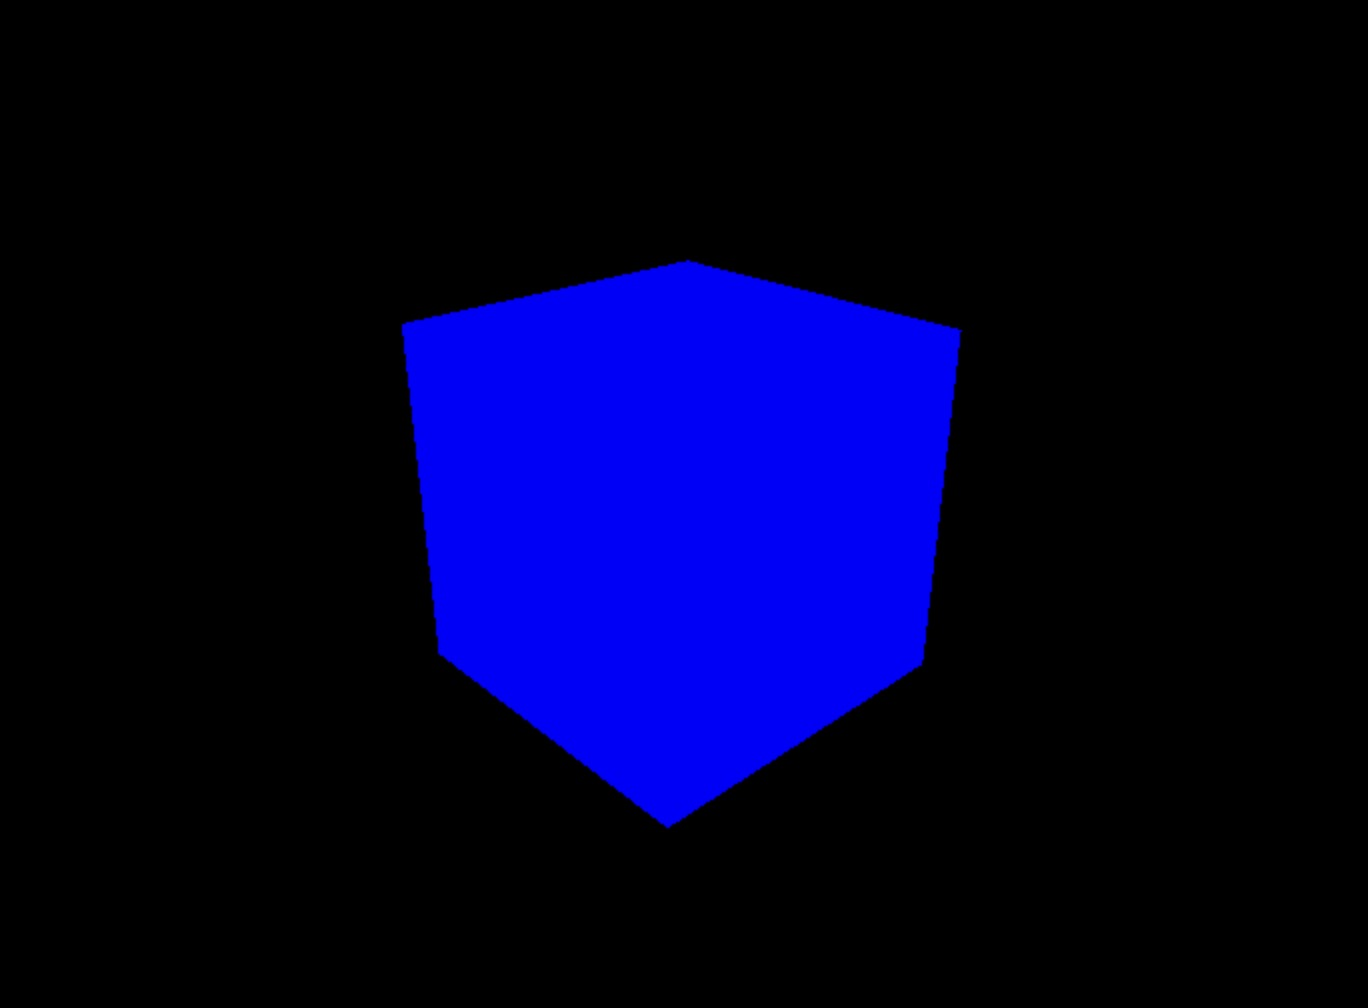
\includegraphics[width=1\linewidth]{graphics/boxGeometry}
\caption[BoxGeometry mesh visualisatie]{BoxGeometry mesh visualisatie}
\label{fig:boxGeometry}
\end{figure}

\newpage
\subsubsection{De camera}

Nu de mesh toegevoegd is aan de scene komt de volgende stap en dat is een camera plaatsen in de scene. De camera is niet zichtbaar en is eerder een theoretisch 'punt' waaruit de render zal plaatsvinden. Er is ook een mogelijkheid om meerdere camera's te gebruiken maar dit is een zeldzaam gegeven. Net zoals er vele soorten geometrieën en materialen zijn, komen ook meerderde soorten camera's voor.

Bij het aanmaken van een camera zijn opnieuw twee vereisten: de 'field of view' of gezichtsveld en de 'aspect ratio' of beeldverhouding. 

Het gezichtsveld is de grootte van de hoek waaruit gekeken wordt, is de hoek groot dan zal alles vervormd worden op een manier dat het uitgezoomd oogt. Als de hoek echter klein is dan lijkt het alsof er ingezoomd word. Een standaard waarde voor het gezichtsveld of 'FOV' is 75 graden en correspondeert met de verticale hoek.

De beeldverhouding wordt in de meeste gevallen bepaald door de breedte te delen door de hoogte. In volgend voorbeeld wordt gedemonstreerd hoe een simpele \texttt{PerspectiveCamera} in de scene geplaatst wordt \autocite{Simon2023}.

\begin{lstlisting}
const maten = {
	breedte: 800,
	hoogte: 600
}

const camera = new THREE.PerspectiveCamera(75, maten.breedte / maten.hoogte)
scene.add(camera)
\end{lstlisting}

\subsubsection{De renderer}

Als laatste moet de scene weergegeven worden en dit kan a.d.h.v. een renderer. Dat doet de renderer door te communiceren met WebGL. Om de render te zien wordt een canvas element meegegeven aan de renderer als volgt: 

\begin{lstlisting}
const canvas = document.querySelector('canvas.webgl')

const renderer = new THREE.WebGLRenderer({ canvas: canvas })
renderer.setSize(maten.breedte, maten.hoogte)

renderer.render(scene, camera)
\end{lstlisting}

Nog een nodige stap om de basis scene te zien is om de camera of de kubus van positie te veranderen omdat ze zich nu allebei in het midden van de scene bevinden. Dit kan simpelweg gedaan worden door de positie property van de camera te veranderen. Het is belangrijk dat deze bewerking uitgevoerd word vooraleer de render uitgevoerd word \autocite{Simon2023}.

\begin{lstlisting}
camera.position.z = 5
\end{lstlisting}

\subsubsection{Transformaties}

Met transformaties kunnen bewerkingen uitgevoerd worden op de meshes die zich bevinden in de scene. Hiervoor zijn er 4 opties: 

\begin{itemize}
	\item positie
	\item schaal
	\item rotatie
	\item kwaternion
\end{itemize}

Deze opties spreken voor zichzelf, de positie bepaald waar de mesh zich bevind in de scene a.d.h.v. de x, y en z eigenschappen. Hiervoor gebruikt Three.js een \texttt{Vector3} klasse, de positie is dus een instantie van de \texttt{Vector3} klasse, zo bestaat er ook de \texttt{Vector2} klasse maar deze is uitzonderlijk toegepast.

De schaal is ook een instantie van de \texttt{Vector3} klasse en heeft dus ook x, y en z eigenschappen.

De rotatie van een mesh is een instantie van Euler i.p.v. \texttt{Vector3} maar heeft ook x, y en z eigenschappen. Euler is een veel gebruikte manier van rotaties noteren in drie-dimensionale omgevingen, als men bijvoorbeeld de mesh 180 graden wil draaien op de x-as kan dat door \texttt{Math.PI} mee te geven aan de x-eigenschap van de rotatie.

Een kwaternion kan ook gebruikt worden om de rotatie van de mesh te bepalen maar is een stuk complexer, het voordeel van de kwaternion is dat het de vaste x, y en z assen vermijd \autocite{Simon2023}.

\subsubsection{Animaties}

Animaties zijn de strekte van Three.js, kort uitgelegd zijn animaties een transformatie uitvoeren op een of meerdere modellen en erna opnieuw een render uitvoeren. Stel dat een kubus zich bevindt op plaats \texttt{(0, 0, 0)} op de initiële render, wanneer de kubus een nieuwe positie krijgt bijvoorbeeld \texttt{(5, 0, 0)} zal de volgende render de kubus zich op de nieuwe positie bevinden. 

Om de animaties er beter te laten uitzien heeft Three.js een oplossing ter beschikking. De klok maakt het gemakkelijk voor developers om goede animaties te maken omdat deze rekening houdt met de tijd die verstreken is. De oorspronkelijke Javascript methode gebruikt de framerate van het scherm van de gebruiker, omdat dit kan verschillen zal geopteerd worden voor de klok \autocite{Simon2023}.

De klok kan als volgt gebruikt worden:
\newpage
\begin{lstlisting}
const klok = new THREE.Clock()

const tick = () =>
{
	const verstrekenTijd = klok.getElapsedTime()
	
	// Update mesh
	mesh.position.x = Math.cos(verstrekenTijd)
}

tick()
\end{lstlisting}

Met de \texttt{getElapsedTime()} methode kan de tijd die verstreken is gevraagd worden, de kubus zal op basis van deze verstreken tijd veranderen van positie. 
\newpage
\subsubsection{Soorten camera's}

Three.js biedt een hoop camera's aan, in dit stuk worden de voornaamste vermeld.

De meeste gebruikte camera is de perspectief camera \ref{fig:perspectiefCamera}, die al eerder vermeld is, hiervoor is een gezichtsveld waarde nodig en een beeldverhouding waarde. De naam van de camera is vanzelfsprekend, wanneer deze gebruikt wordt dan zal de scene vanuit een perspectief bekeken worden. Dat wil zeggen dat het bekeken wordt vanaf 1 punt en waar dat punt is zal bepalen hoe de scene gerendered word.

De orthografische camera \ref{fig:orthografischeCamera} is een andere mogelijkheid, deze camera zal objecten renderen zodat de afstand van het object tot de camera geen invloed heeft op de grootte. Dit kan handig zijn voor 2D scenes of UI elementen te renderen \autocite{threejs2023}.

\begin{figure}[h]
	\centering
	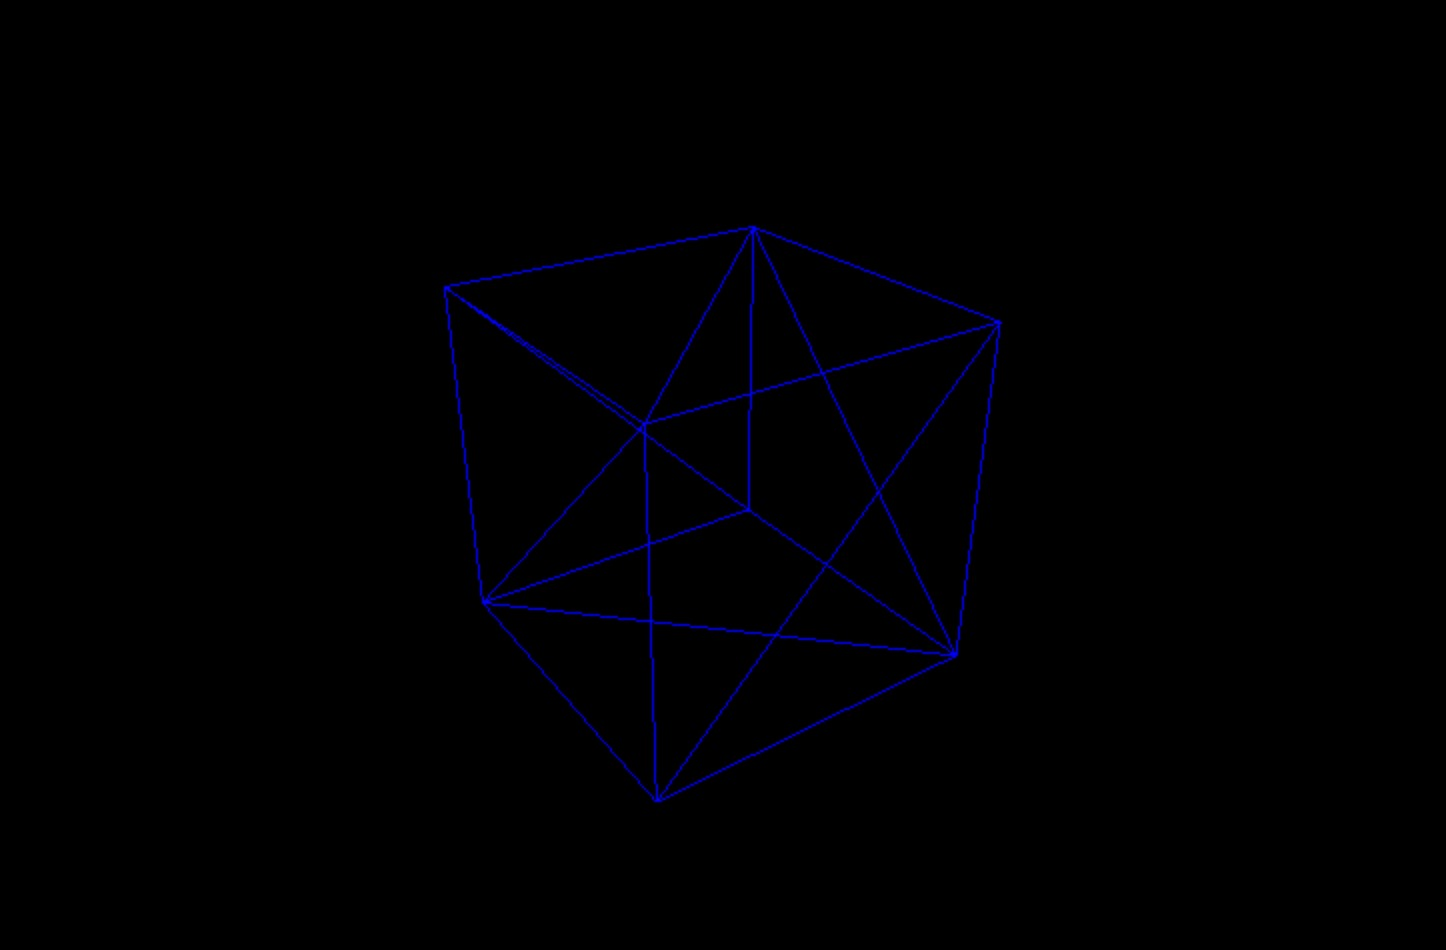
\includegraphics[width=1\linewidth]{graphics/perspectiefCamera}
	\caption[Perspectief camera visualisatie]{Perspectief camera visualisatie wireframe BoxGeometry}
	\label{fig:perspectiefCamera}
\end{figure}

\begin{figure}
	\centering
	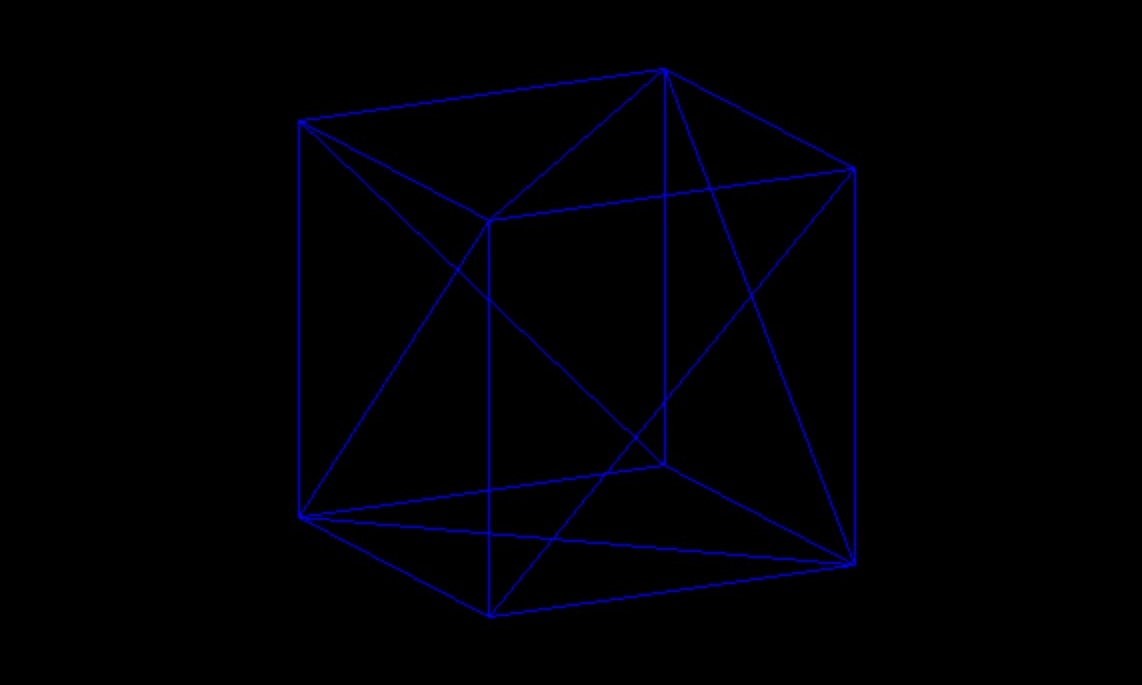
\includegraphics[width=1\linewidth]{graphics/orthografischeCamera}
	\caption[Orthografische camera visualisatie]{Orthografische camera visualisatie wireframe BoxGeometry}
	\label{fig:orthografischeCamera}
\end{figure}
\newpage
\subsubsection{Soorten geometriën}

De bibliotheek van Three.js heeft een veel basis geometriën waar developers gemakkelijk van gebruik kunnen maken. Tijdens het schrijven van deze scriptie zijn er 18 ter beschikking waaronder de \texttt{BoxGeometry} \ref{fig:boxGeometry}, \texttt{PlaneGeometry} \ref{fig:planeGeometry}, \texttt{SphereGeometry} \ref{fig:sphereGeometry}, \texttt{TextGeometry} en nog meer.

Een geometrie in Three.js bestaat uit vertices en vlakken. Elke geometrie heeft in essentie een hoop driehoeken met 3 vertices of hoekpunten en een vlak. Wanneer deze driehoeken gecombineerd worden geeft het als resultaat een geometrie. Hiermee kan Three.js zeer complexe maar ook zeer simpele vormen representeren. Als voorbeeld kan een vlak genomen worden of in Three.js genaamd een \texttt{PlaneGeometry} \ref{fig:planeGeometry}, een vlak bestaat uit twee driehoeken en heeft dus 6 vertices. Een stap hoger is dan de \texttt{BoxGeometry} \ref{fig:boxGeometry} die 6 vlakken omvat en dus uit 12 driehoeken of 36 vertices bestaat. Nog een paar stappen hoger en dan kan een \texttt{SphereGeometry} \ref{fig:sphereGeometry} gemaakt worden, deze vorm is een stuk complexer. Het lijkt alsof de mesh het een bol is maar in realiteit bestaat de bol uit een hoop vlakken en heeft dus veel meer driehoeken nodig om gerealiseerd te worden \autocite{threejs2023}.

Hoe meer driehoeken er gebruikt worden hoe meer detail de developer dus kan implementeren maar dit brengt een prijs met zich mee. Elke vertex heeft een coördinaat en moet gerendered worden, wanneer er animaties gebeuren in de scene en de developer is iets te enthousiast geweest dan kan al zeer snel een vertaging zijn. Zeker als we weten dat er nog veel computers zijn waar de GPU nog niet optimaal is, bijvoorbeeld op gsm's. Wanneer men dus met animaties werkt is het vaak een vuistregel om zo weinig mogelijk driehoeken te gebruiken voor de geometriën. Zo kan de beste omgeving voorzien worden om elke gebruiker de optimale ervaring te geven.

\begin{figure}[h]
	\centering
	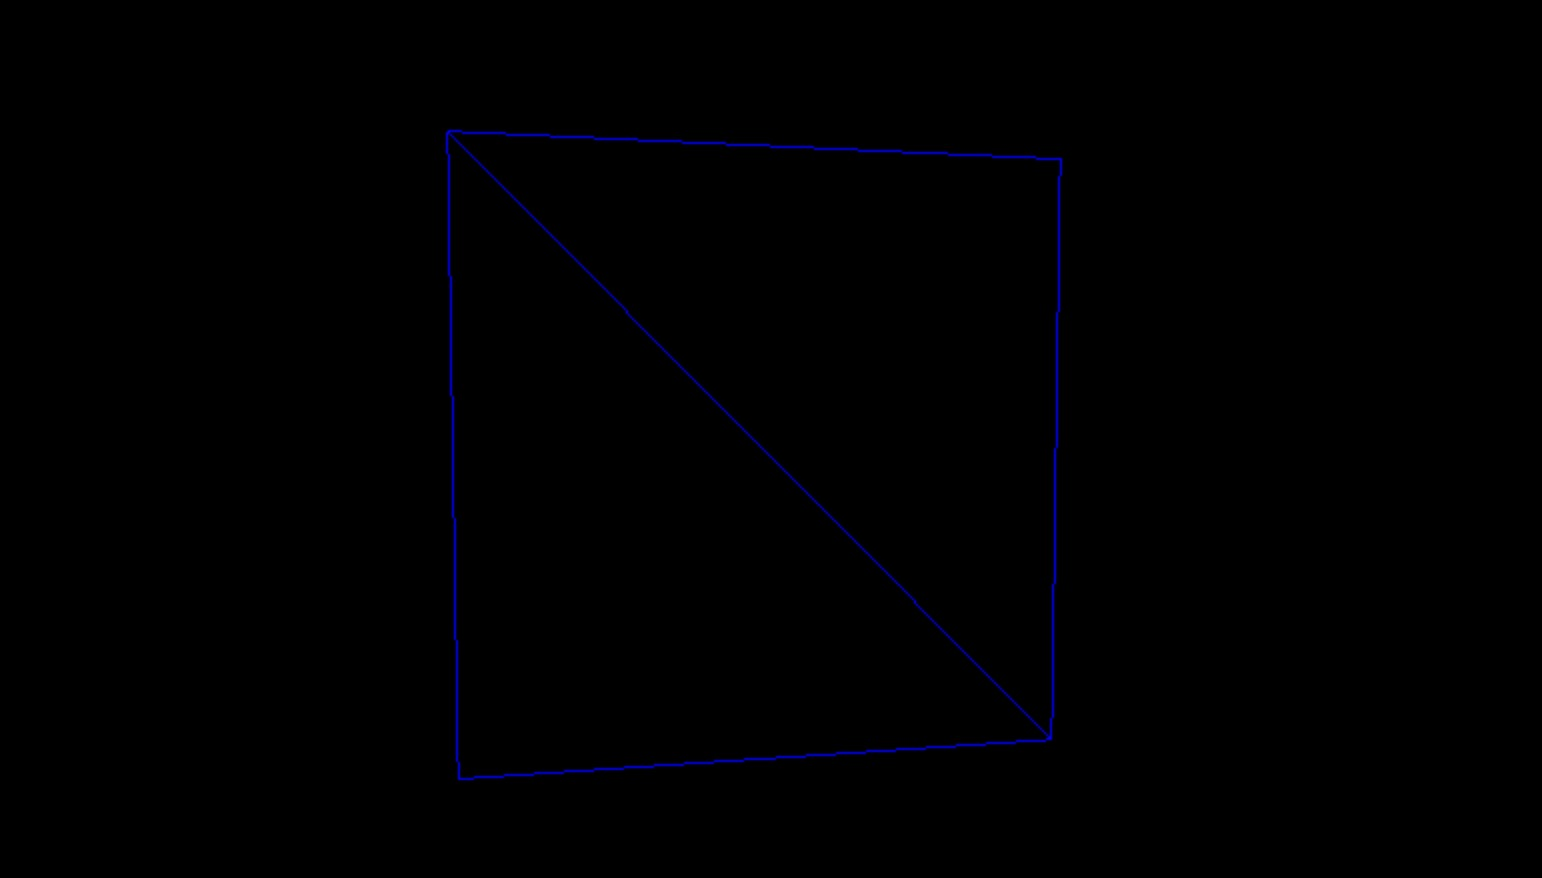
\includegraphics[width=.7\linewidth]{graphics/planeGeometry}
	\caption[Visualisatie wireframe PlaneGeometry]{Visualisatie wireframe PlaneGeometry}
	\label{fig:planeGeometry}
\end{figure}

\begin{figure}[h]
	\centering
	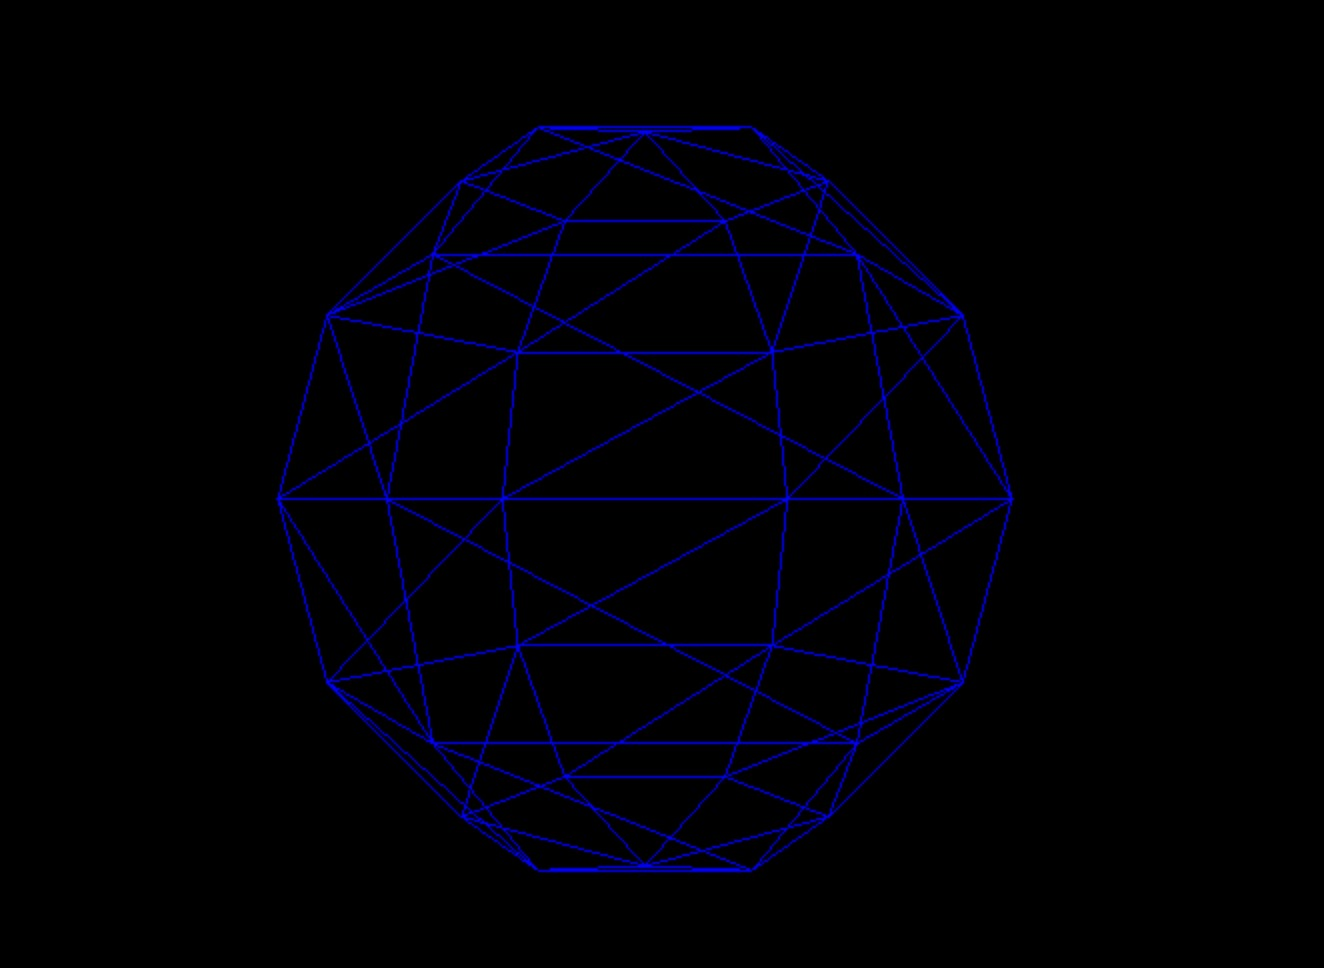
\includegraphics[width=.7\linewidth]{graphics/sphereGeometry}
	\caption[Visualisatie wireframe SphereGeometry]{Visualisatie wireframe SphereGeometry}
	\label{fig:sphereGeometry}
\end{figure}

\newpage
\subsubsection{Texturen}

Texturen zijn afbeeldingen die over de vlakken van een geometrie gelegd worden. Hierbij bestaan de volgende soorten texturen: 

\begin{itemize}
\item Kleur of albedo
\item Alfa
\item Hoogte
\item Normaal
\item Omgevingsocclusie
\item Metaalheid
\item Ruwheid
\end{itemize}

Deze texturen bieden de mogelijkheid aan om een geometrie een realistisch uitzicht te geven. Met de kleur textuur \ref{fig:colorTexture} zal elke pixel van de afbeelding geplakt worden op de geometrie. De alfa textuur \ref{fig:alphaTexture} is een grijstint afbeelding waar wit het zichtbare voorstelt en zwart hetgeen wat niet zichtbaar is. De hoogte textuur \ref{fig:heightTexture} is ook een grijstint afbeelding die a.d.h.v. de tinten een reliëf creëert in de geometrie. Hierbij zullen de vertices van plaats veranderd worden om dit effect te verwezenlijken. De normaal textuur \ref{fig:normalTexture} voegt kleine details toe aan de geometrie en doet dit door het licht zodanig te manipuleren dat het denkt dat bepaalde vlakken of driehoeken anders georiënteerd zijn. De omgevingsocclusie textuur \ref{fig:ambientOcclusionTexture} is opnieuw een grijstint afbeelding die valse schaduwen zal plakken in de gleuven van de geometrie, alhoewel deze schaduwen niet echt zijn zorgt het voor een beter contrast. Met de metaaheid textuur \ref{fig:metalnessTexture}, dat ook een grijstint afbeelding is, zullen de stukken van de geometrie die metaal zijn in het wit voorgesteld worden. Met deze info maakt Three.js deze delen van de geometrie reflectief. En dan is er tenslotte de ruwheid textuur \ref{fig:roughnessTexture} die grijstinten gebruikt om op dezelfde manier als de metaalheid textuur delen van de geometrie een ruwheid te geven \autocite{Simon2023}.

Omdat texturen eigenlijk afbeeldingen zijn worden ze met normale Javascript code ingeladen om dan in Three.js als volgt gedefinieerd te worden:

\begin{lstlisting}
const textuur = new THREE.Texture(afbeelding)
\end{lstlisting}

\begin{figure}[]
	\centering
	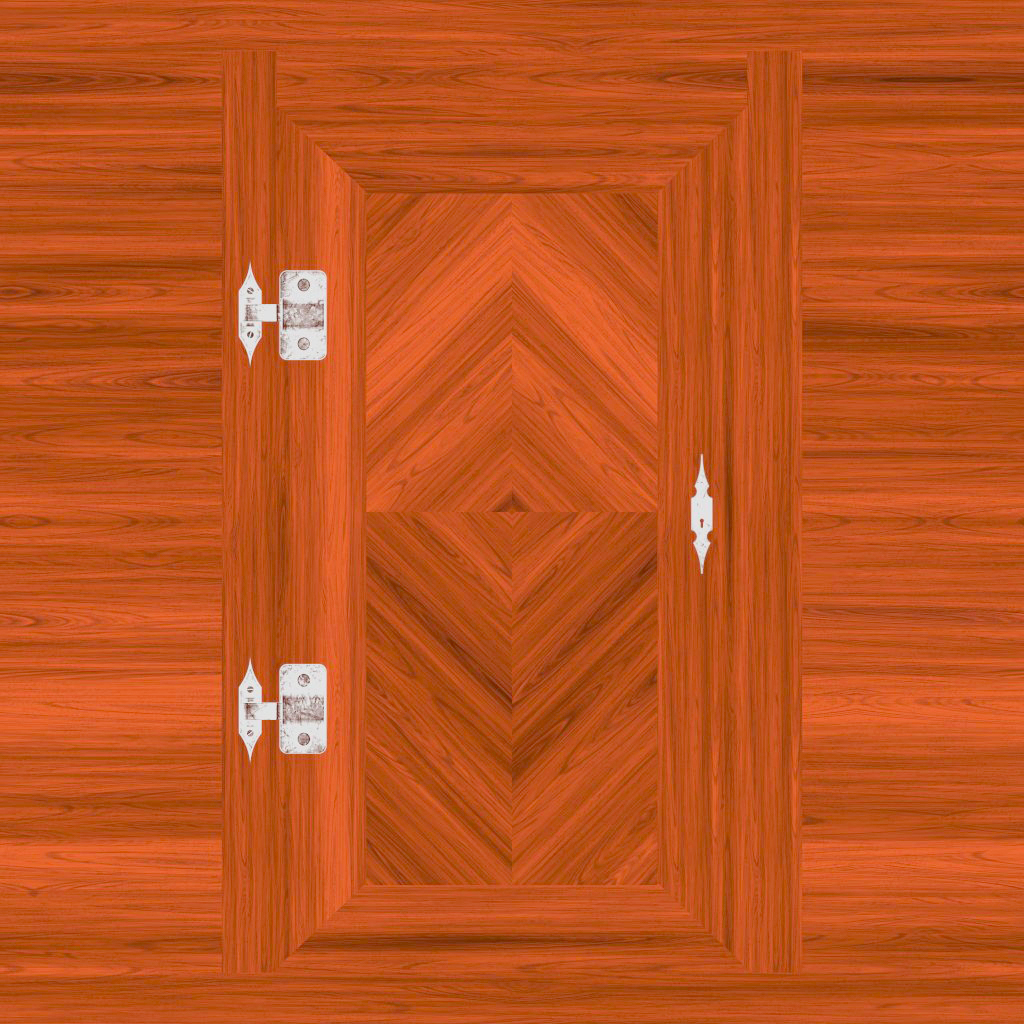
\includegraphics[width=.5\linewidth]{graphics/colorTexture}
	\caption[Kleur textuur afbeelding]{Kleur textuur afbeelding}
	\label{fig:colorTexture}
\end{figure}
\begin{figure}[]
	\centering
	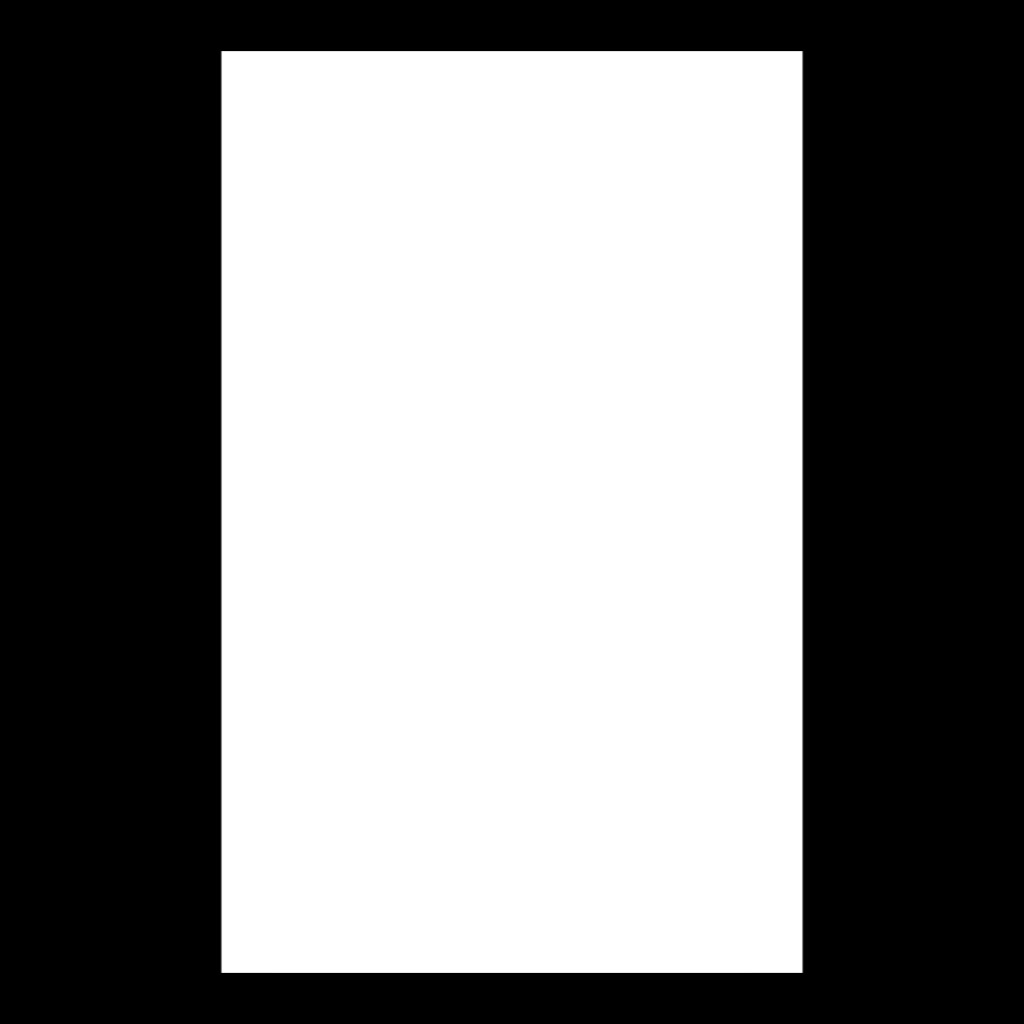
\includegraphics[width=.5\linewidth]{graphics/alphaTexture}
	\caption[Alfa textuur]{Alfa textuur}
	\label{fig:alphaTexture}
\end{figure}
\begin{figure}[]
	\centering
	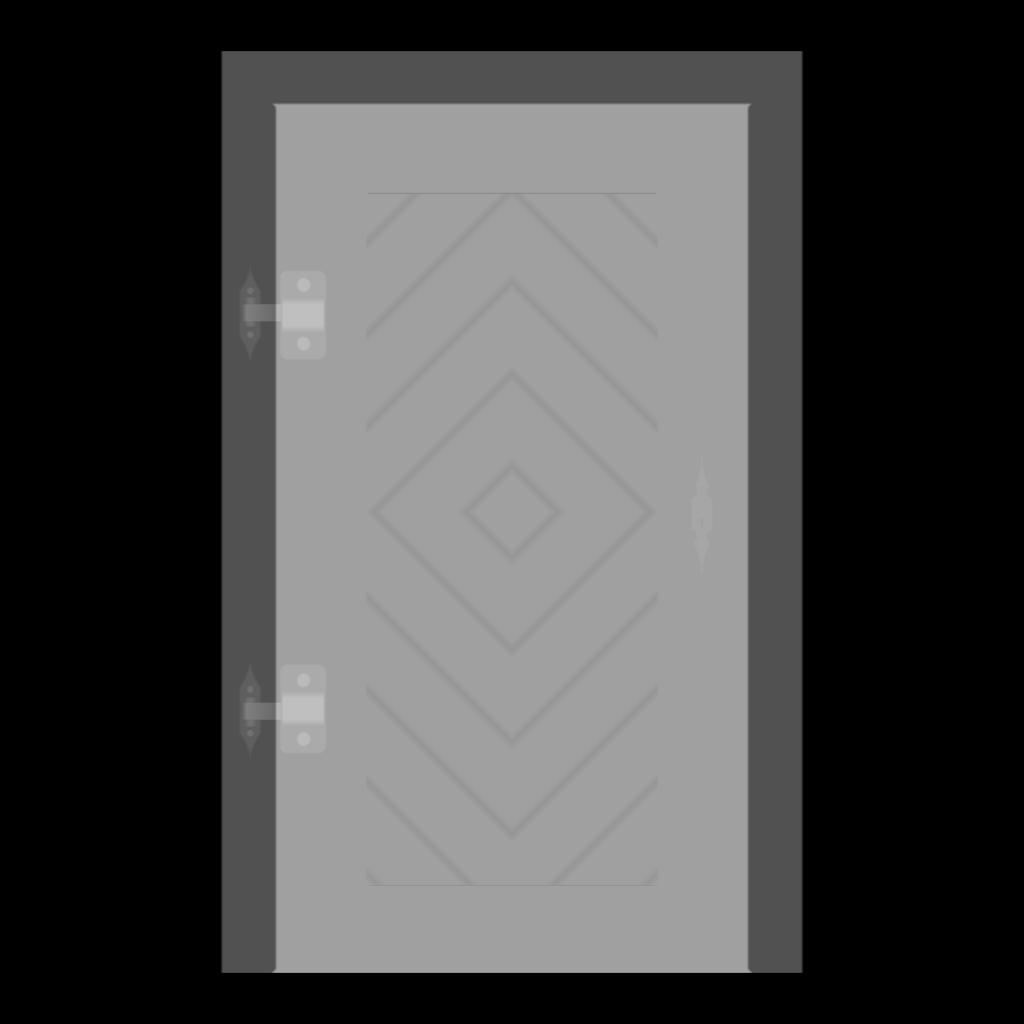
\includegraphics[width=.5\linewidth]{graphics/heightTexture}
	\caption[Hoogte textuur]{Hoogte textuur}
	\label{fig:heightTexture}
\end{figure}
\begin{figure}[]
	\centering
	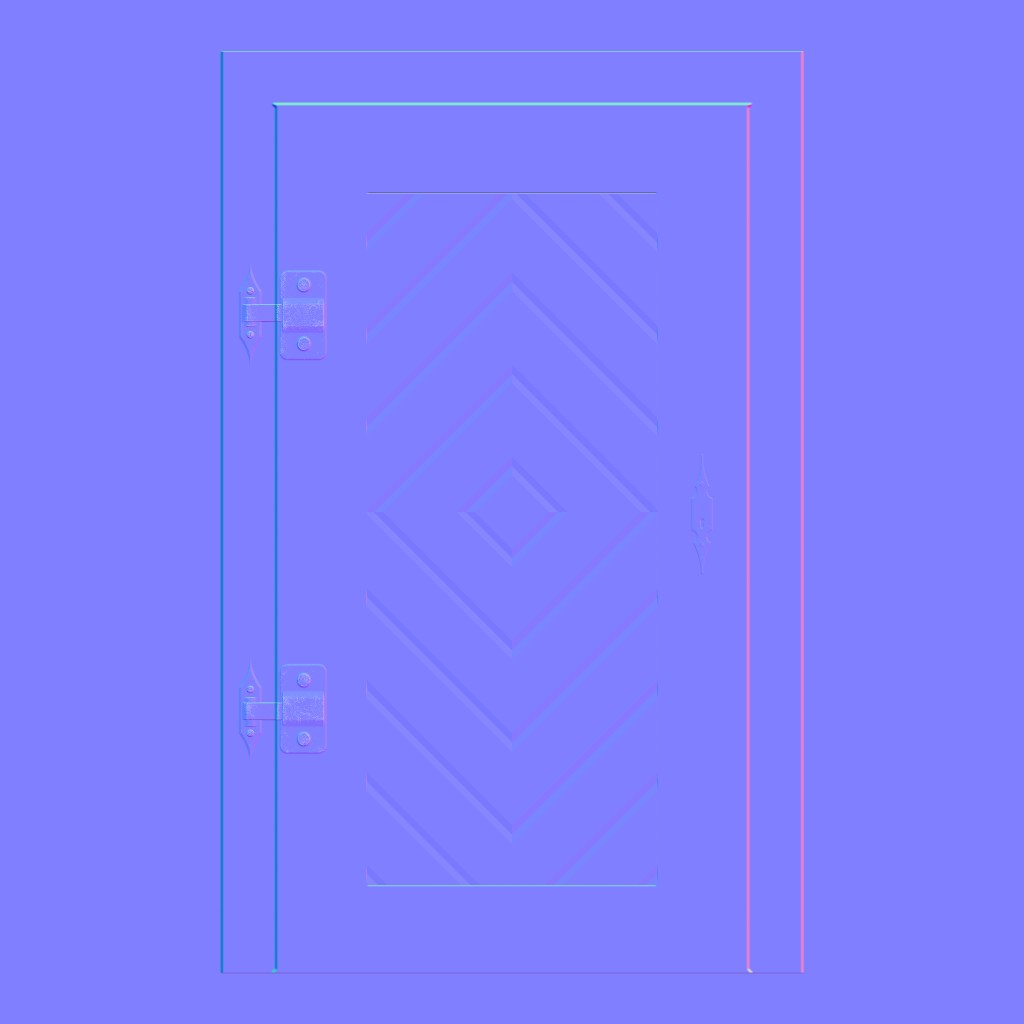
\includegraphics[width=.5\linewidth]{graphics/normalTexture}
	\caption[Normaal textuur]{Normaal textuur}
	\label{fig:normalTexture}
\end{figure}
\begin{figure}[]
	\centering
	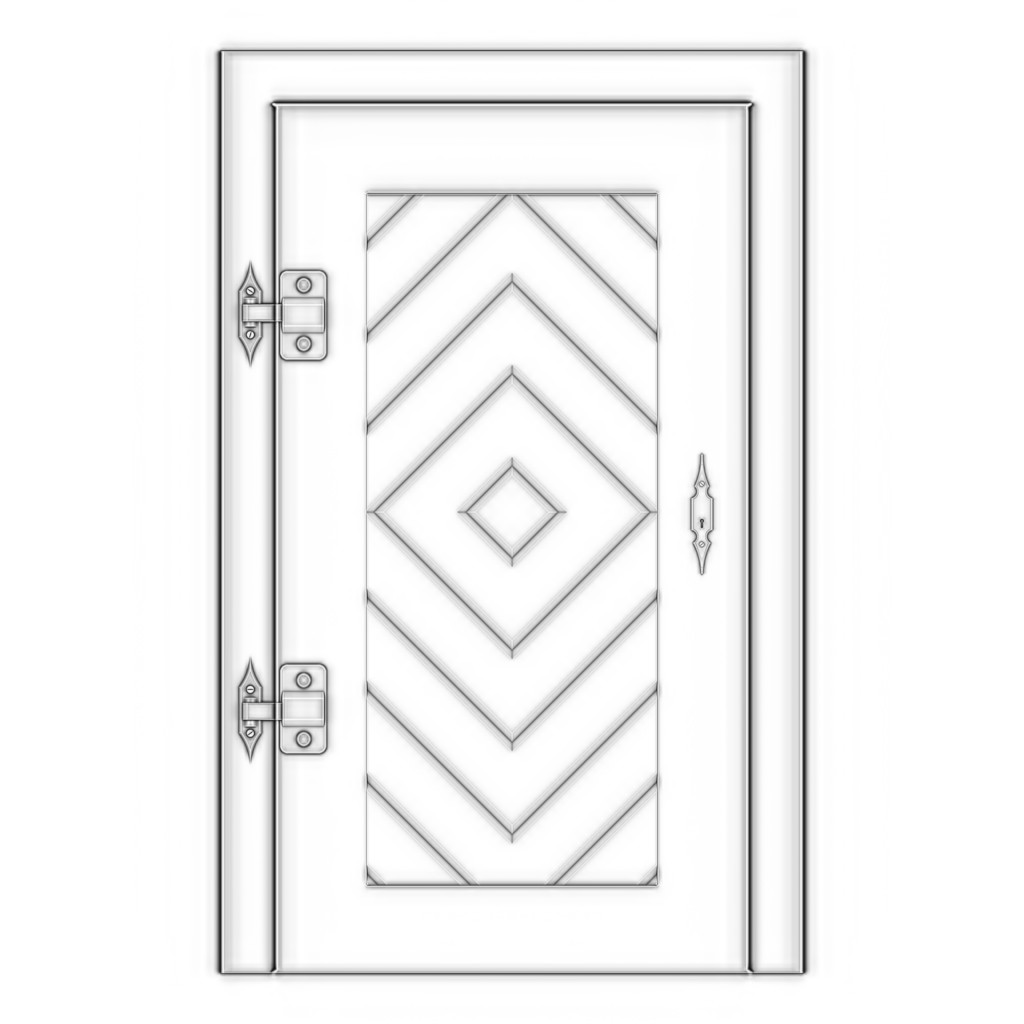
\includegraphics[width=.5\linewidth]{graphics/ambientOcclusionTexture}
	\caption[OmgevingsOcclusie textuur]{OmgevingsOcclusie textuur}
	\label{fig:ambientOcclusionTexture}
\end{figure}
\begin{figure}[]
	\centering
	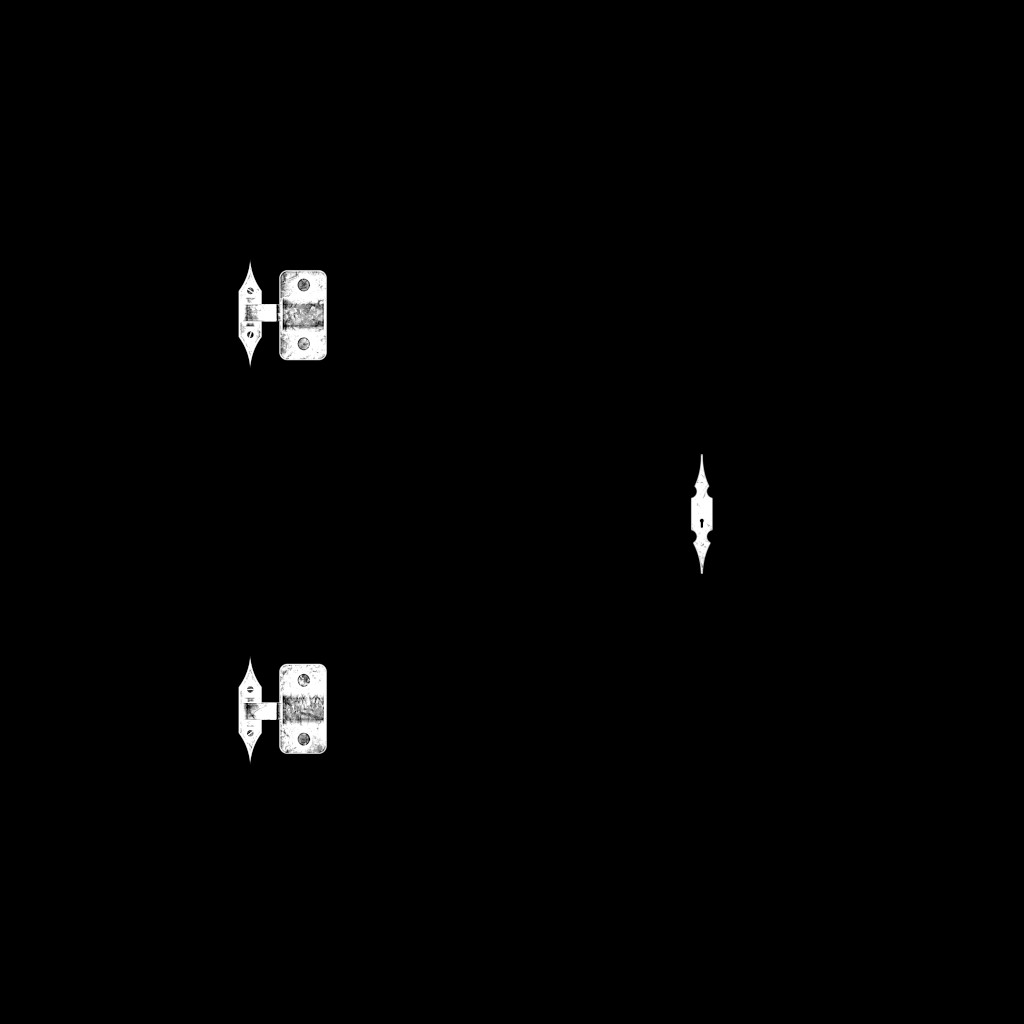
\includegraphics[width=.5\linewidth]{graphics/metalnessTexture}
	\caption[Metaalheid textuur]{Metaalheid textuur}
	\label{fig:metalnessTexture}
\end{figure}
\begin{figure}[]
	\centering
	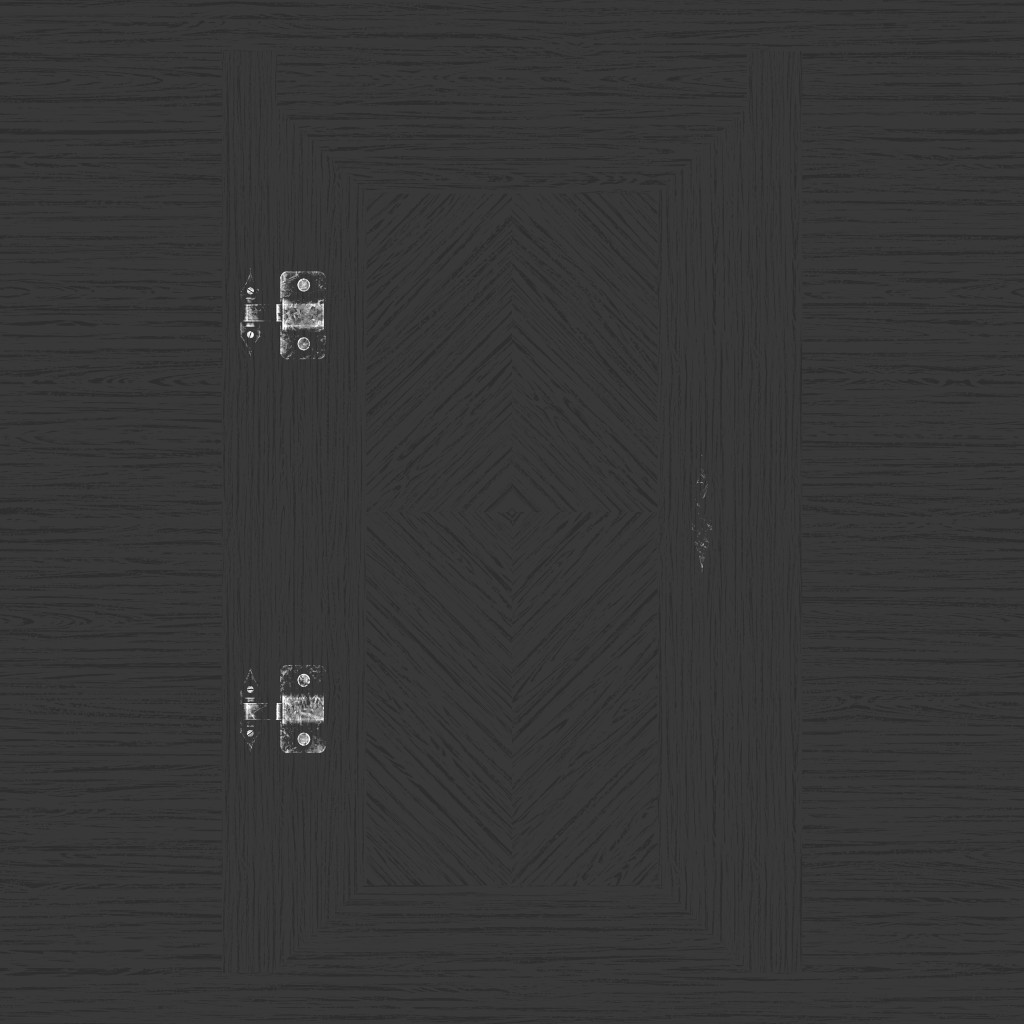
\includegraphics[width=.5\linewidth]{graphics/roughnessTexture}
	\caption[Ruwheid textuur]{Ruwheid textuur}
	\label{fig:roughnessTexture}
\end{figure}

\newpage
\subsubsection{Materialen}

Materialen worden in Three.js gebruikt om een kleur te voorzien voor elke zichtbare pixel van een geometrie. De algoritmes die bepalen welke pixel welke kleur krijgt zijn geschreven in specifieke 'shader' programma's. Shaders schrijven is een uiterst complex gegeven en is dus zeker niet voor iedereen weggelegd maar gelukkig biedt Three.js materialen aan met ingebouwde shaders \autocite{Simon2023}.

Een materiaal zal de textuur mappen op de geometrie en daarvoor hoeft de developer niet veel te doen. Het kan op de volgende manier gedaan worden:

\begin{lstlisting}
const materiaal = new THREE.MeshBasicMaterial({ map: textuur })
\end{lstlisting}

Voor de verschillende soorten texturen zijn ook methodes voorzien om ze correct te plaatsen op de geometrie.

\subsubsection{Tekst geometrie}

De tekst geometrie genereert kort gezegd 3D tekst. Deze geometrie werkt bijna exact hetzelfde als de andere en wordt gebruikt om tekst te plaatsen in een scene. De extra stap die genomen moet worden is om een font mee te geven bij de initialisatie, daarvoor moet eerst een \texttt{FontLoader} aangemaakt worden om de font in te laden. Vervolgens kan dan de font ingeladen worden.

\begin{lstlisting}
const fontLoader = new THREE.FontLoader()

// Inladen font
const fontKeuze = fontloader.load('/fonts/fontNaarKeuze.typeface.json')
\end{lstlisting}

Nu de font ingeladen is kan de tekst geometrie geïnitialiseerd en uiteraard ook toegevoegd worden aan de scene. Dit wordt als volgt gedaan:

\begin{lstlisting}
const textGeometrie = new THREE.TextGeometry('Hello World', { font: fontKeuze })
const textMateriaal = new THREE.MeshBasicMaterial()

const text = new THREE.Mesh(textGeometrie, textMateriaal)
scene.add(text)
\end{lstlisting}

\newpage
\subsection{Klassieke Technieken}

In dit hoofdstuk worden de technieken overlopen in Three.js die niet noodzakelijk zijn om een scene te maken maar wel zorgen voor een aanzienlijke meerwaarde.

\subsubsection{Lichten}

Met licht kan in een scene een compleet ander perspectief gegeven worden aan meshes. Hierbij zijn er een aantal lichten die ter beschikking gesteld zijn waaronder:

\begin{itemize}
	\item AmbientLight
	\item DirectionalLight
	\item HemisphereLight
	\item PointLight
	\item RectAreaLight
	\item SpotLight
\end{itemize}

Omdat \texttt{AmbientLight} of omgevingslicht en \texttt{DirectionalLight} of directioneel licht de voornaamste zijn die gebruikt worden binnen Three.js zullen deze uitgediept worden. Uitleg over de andere soorten licht is te vinden op de documentatie van Three.js.

Belangrijk is dat materialen verschillend kunnen reageren op licht, het \newline \texttt{MeshBasicMaterial} is bijvoorbeeld niet beïnvloed door licht. Er moet dus een ander soort materiaal gebruikt worden, hiervoor kan \texttt{MeshStandardMaterial} op de mesh toegepast worden. Bij dit materiaal is het noodzakelijk om een licht te gebruiken want indien er geen licht aanwezig is in de scene, dan zal de mesh ook niet zichtbaar zijn \autocite{Simon2023}.

\subsubsection{AmbientLight}

AmbientLight of omgevingslicht \ref{fig:ambientLight}  geeft omnidirectioneel licht op alle meshes die zich in de scene bevinden. Het initialiseren van dit licht vergt twee parameters zijnde de kleur en intensiteit.

\begin{lstlisting}
const omgevingslicht = new THREE.AmbientLight(0xffffff, 0.5)
scene.add(omgevingslicht)
\end{lstlisting}

\subsubsection{DirectionalLight}

\texttt{DirectionalLight} of directioneel licht \ref{fig:directionalLight} kan vergeleken worden met zonlicht, alle stralen komen parallel vanuit dezelfde richting maar geen specifiek punt. Hierbij kan de positie aangepast worden net zoals de positie van de zon ook kan veranderen, bij initialisatie wordt ook de kleur en intensiteit meegegeven.

\begin{lstlisting}
const directioneelLicht = new THREE.DirectionalLight(0x00fffc, 0.4)
scene.add(directioneelLicht)
\end{lstlisting}

De positie kan op de volgende eenvoudige manier na initialisatie veranderd worden.

\begin{lstlisting}
directioneelLicht.position.set(1, .5, 0)
\end{lstlisting}

\begin{figure}[h]
	\centering
	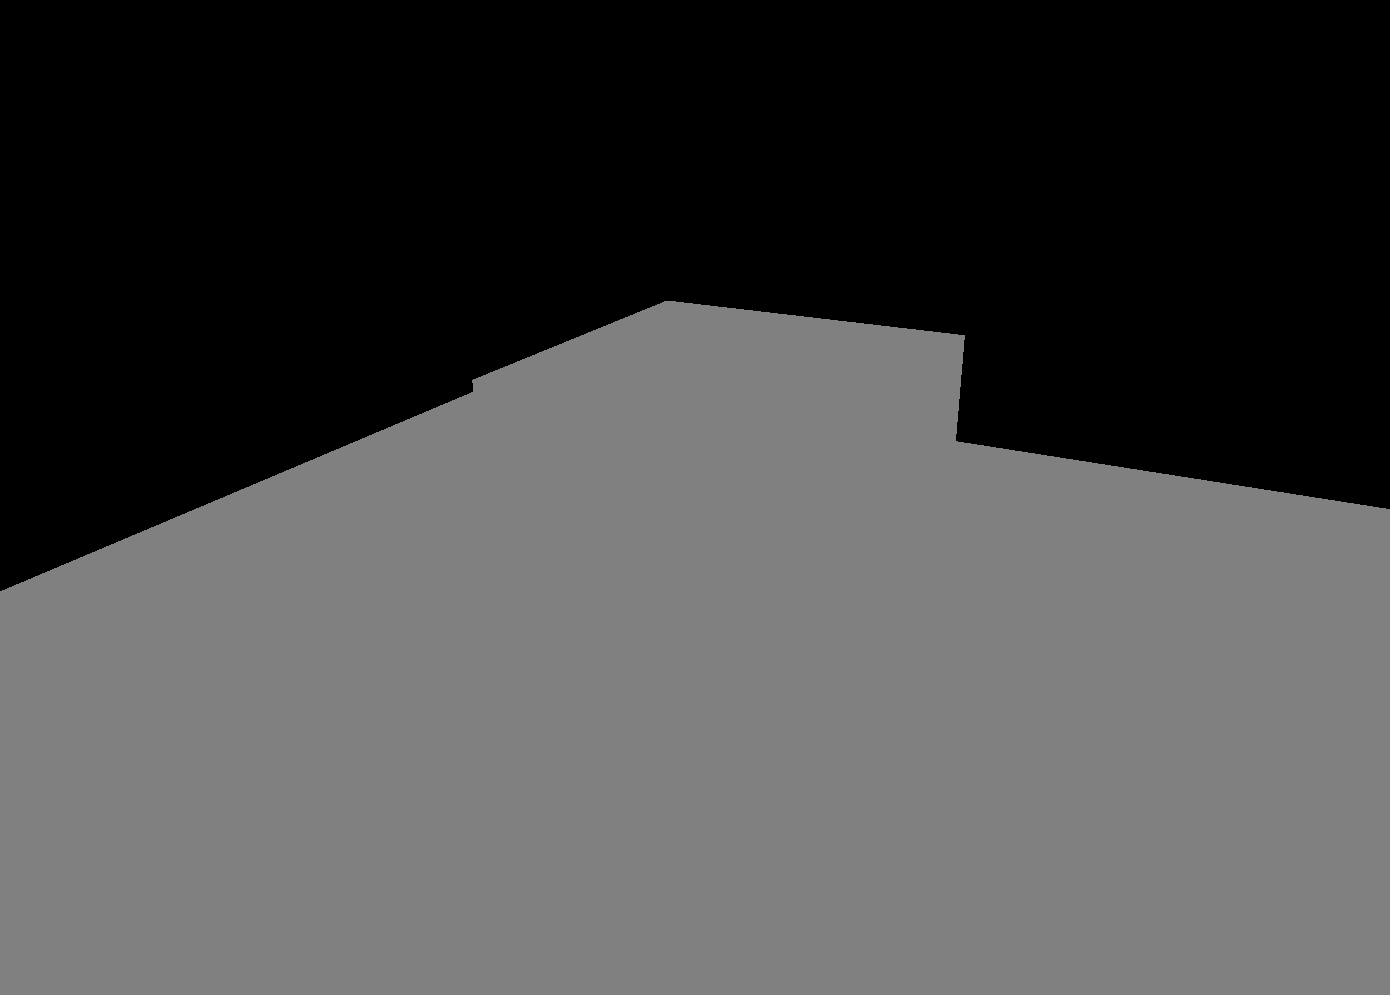
\includegraphics[width=.7\linewidth]{graphics/ambientLight}
	\caption[Omgevingslicht voorbeeld van BoxGeometry en PlaneGeometry]{Omgevingslicht voorbeeld van BoxGeometry en PlaneGeometry}
	\label{fig:ambientLight}
\end{figure}

\begin{figure}[h]
	\centering
	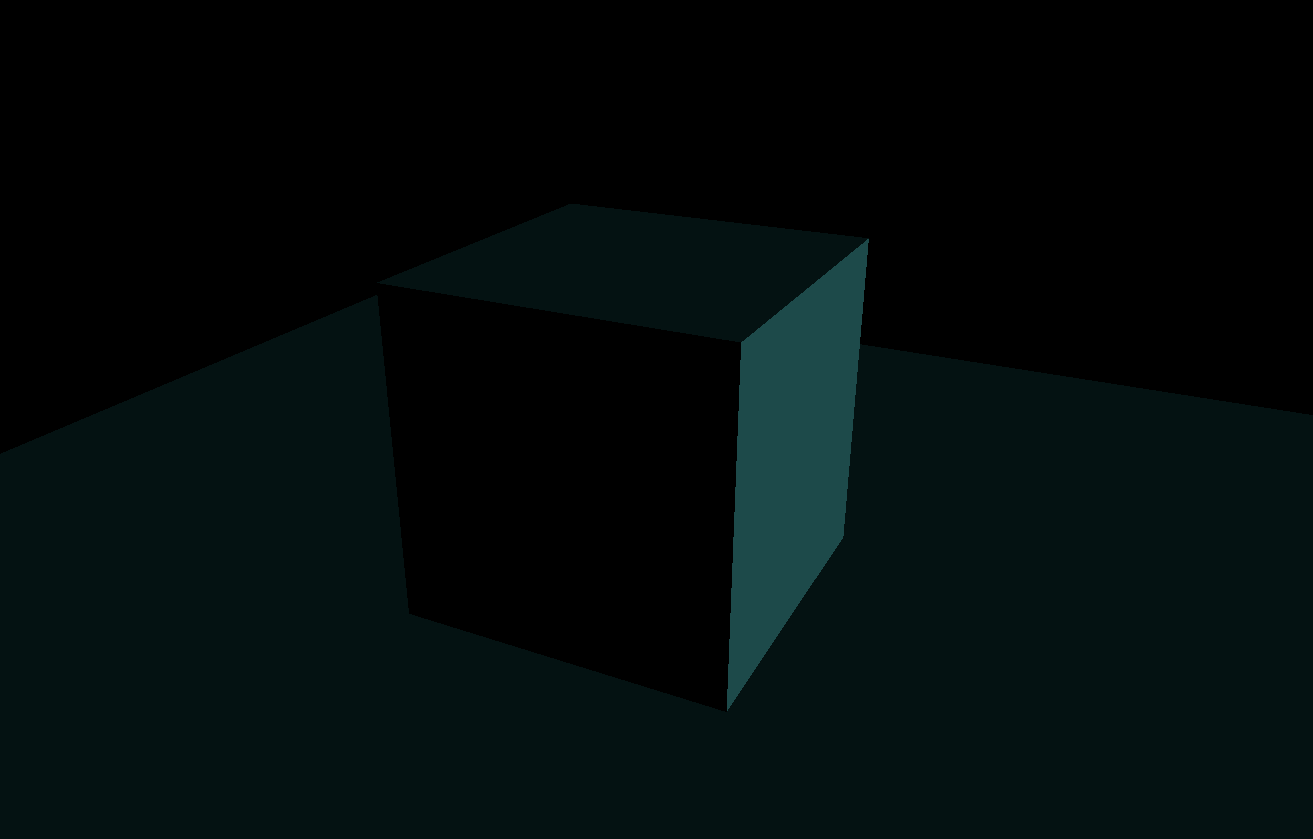
\includegraphics[width=.7\linewidth]{graphics/directionalLight}
	\caption[Directioneel licht voorbeeld van BoxGeometry en PlaneGeometry]{Directioneel licht voorbeeld van BoxGeometry en PlaneGeometry}
	\label{fig:directionalLight}
\end{figure}
\newpage
Lichten kunnen ook gecombineerd worden om een realistisch beeld te verkrijgen, zie Figuur  \ref{fig:ambientPlusDirectionalLight}  \autocite{Simon2023}.

\begin{figure}[h]
	\centering
	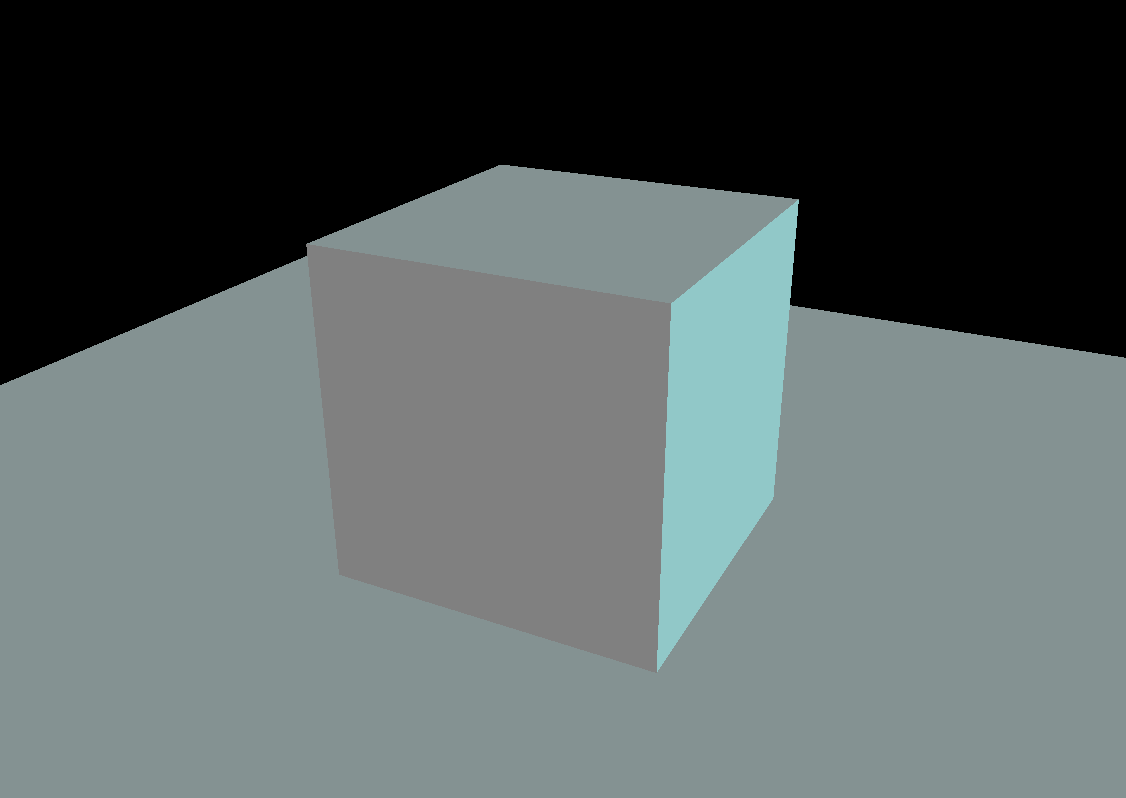
\includegraphics[width=.7\linewidth]{graphics/ambientPlusDirectionalLight}
	\caption[Voorbeeld omgevingslicht plus directioneel licht]{Voorbeeld omgevingslicht plus directioneel licht}
	\label{fig:ambientPlusDirectionalLight}
\end{figure}

\subsubsection{Helpers}

Omdat het soms moeilijk kan zijn om een goed beeld te krijgen over waar een licht zich in de scene bevind kan het handig zijn om een helper te gebruiken. Deze dient als een hulplijn om de gewenste positie en dus resultaat te verkrijgen. Zie figuur \ref{fig:directionalLightHelper} voor een voorbeeld van een directioneel licht helper.

\begin{figure}[h]
	\centering
	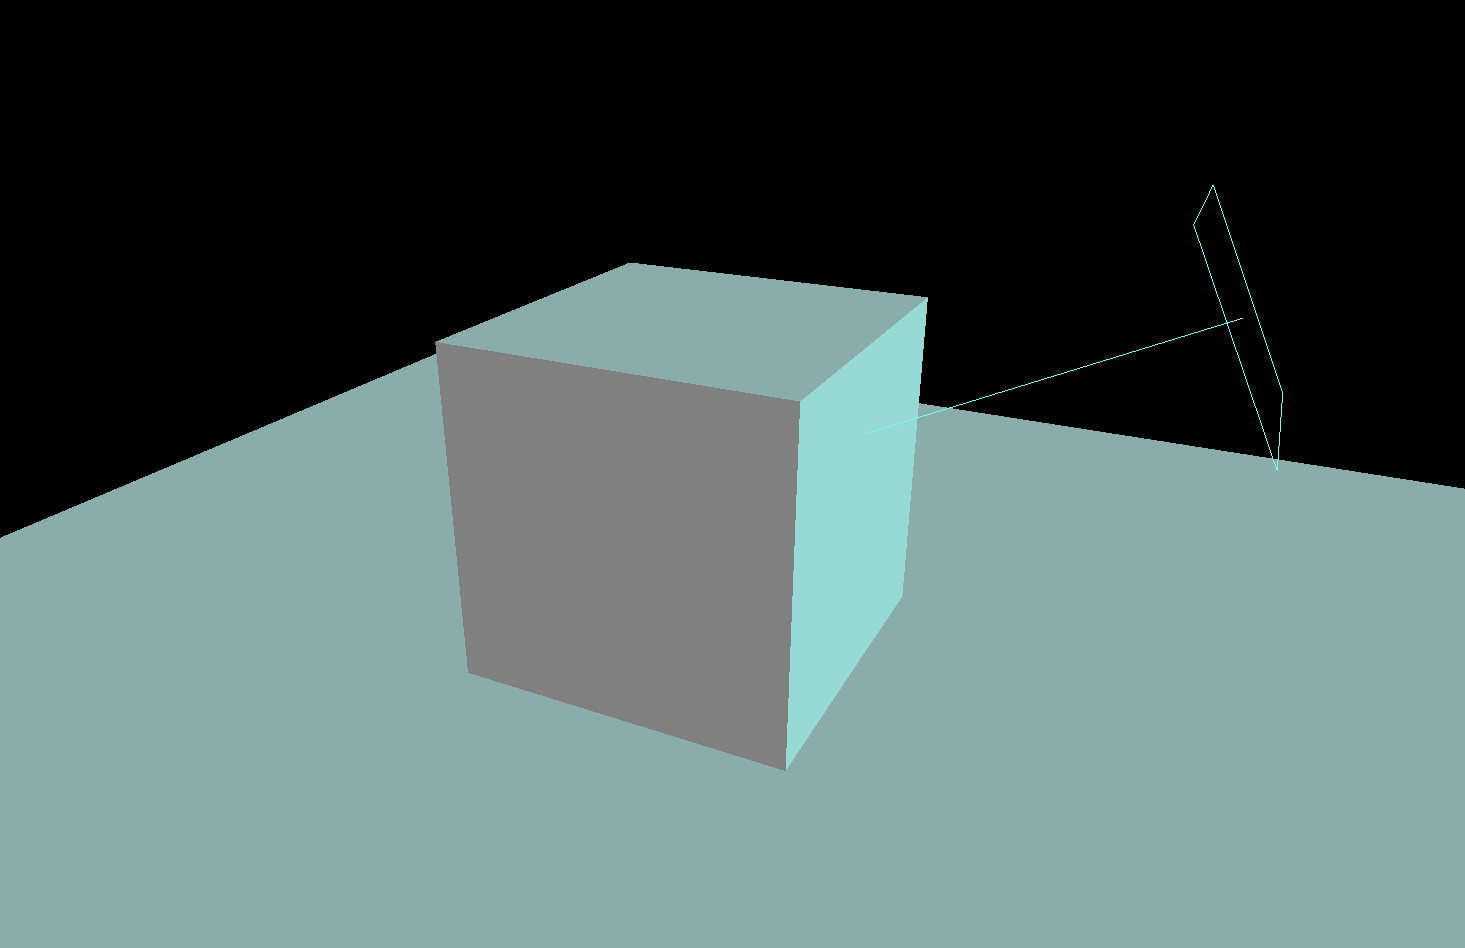
\includegraphics[width=.7\linewidth]{graphics/directionalLightHelper}
	\caption[Voorbeeld omgevingslicht plus directioneel licht met helper]{Voorbeeld omgevingslicht plus directioneel licht met helper}
	\label{fig:directionalLightHelper}
\end{figure}

\subsubsection{Schaduwen}

Met de inbreng van licht krijgen we uiteraard ook schaduwen waarbij de achterkant van objecten donker wordt, wat bekend staat als de kernschaduw. Hetgeen wat nog mist is de slagschaduw, hierbij zorgen meshes voor schaduwen op andere meshes.

De keerzijde van het implementeren van schaduwen is dat ze moeilijk te verkrijgen zijn aan een optimale frame rate. Developers zullen dus creatieve oplossingen moeten vinden om een degelijke frame rate te verkrijgen \autocite{Simon2023}.

Er zijn drie soorten lichten die het gebruik van slagschaduwen mogelijk maken, deze zijn \texttt{DirectionalLight}, \texttt{PointLight} en \texttt{SpotLight}. In deze scriptie zal alleen \texttt{DirectionalLight} behandeld worden.

De schaduwen moeten eerst als volgt aangezet worden:

\begin{lstlisting}
renderer.shadowMap.enabled = true
\end{lstlisting}

Vervolgens moet doorheen elk object in de scene gegaan worden en bepaald worden of de mesh een schaduw moet maken, krijgen of beide. Dit moet ook bepaald worden voor het licht.

\begin{lstlisting}
mesh.castShadow = true
mesh.receiveShadow = true

directioneelLicht.castShadow = true
\end{lstlisting}

Zie figuur \ref{fig:shadow} voor een voorbeeld van het schaduw effect.

Voor performantie is de standaard waarde voor de schaduw map 512x512, voor meer gedetailleerde schaduwen kan de schaduw map grootte verhoogd worden met een macht van twee.

\begin{lstlisting}
directioneelLicht.shadow.mapSize.width = 1024
directioneelLicht.shadow.mapSize.height = 1024
\end{lstlisting}

Over schaduwen kan nog veel meer gezegd worden. Zo kan men bijvoorbeeld i.p.v. de schaduw te genereren een versie 'bakken' in een afbeelding en de op de mesh plakken, maar dit is al een stuk geavanceerder \autocite{Simon2023}.

\begin{figure}
	\centering
	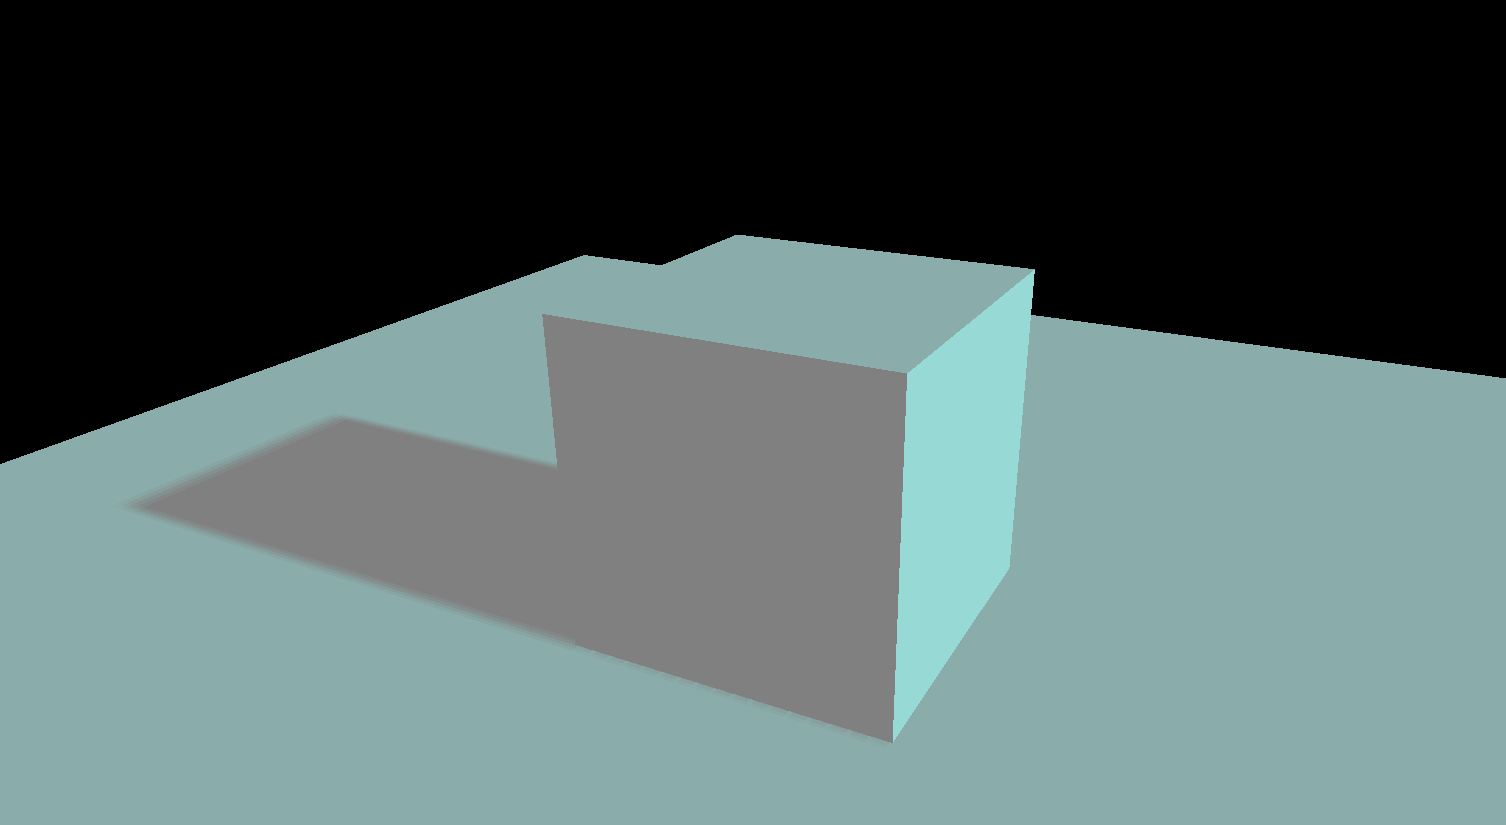
\includegraphics[width=1\linewidth]{graphics/shadow}
	\caption[Voorbeeld omgevingslicht plus directioneel licht met slagschaduw]{Voorbeeld omgevingslicht plus directioneel licht met slagschaduw}
	\label{fig:shadow}
\end{figure}

\subsubsection{Fysica}

Fysica implementeren in een scene kan veel interactie geven aan de gebruiker. Zwaartekracht krijgt hier de hoofdrol en zal botsingen tussen de meshes veroorzaken. Dit gebeurd echter niet in een normale scene maar in een aparte wereld waar de krachten gesimuleerd worden. Deze wereld is puur theoretisch en kan niet gezien worden. Wanneer er een mesh wordt aangemaakt zal dezelfde versie van de mesh geïnitialiseerd worden in de natuurkundige wereld.
Op elke frame voor de render is uitgevoerd zal deze wereld een update krijgen en worden de nieuwe coördinaten van de mesh gelijk gemaakt aan de mesh in de normale scene. Dit is de enige vereiste \autocite{Simon2023}.
\newpage
\subsection{React Three Fiber}

React Three Fiber is een bibliotheek die Three.js en React combineert zonder limieten, alles dat werkt in Three.js kan dus ook werken a.d.h.v. R3F. De manier hoe het werkt is dat Three.js vertaald wordt naar JSX, \texttt{<mesh />} zal automatisch veranderen in \texttt{new THREE.Mesh()} \autocite{reactThreeFiber2023}.

\subsubsection{Canvas}

Via het \texttt{Canvas} object geeft R3F toegang tot de Three.js bibliotheek door een scene en renderer aan te maken. Binnen in het  \texttt{Canvas} object kunnen dan alle andere delen geplaatst worden om een volledige ervaring te maken. In volgend voorbeeld word een  \texttt{Canvas} object gebruikt in een React omgeving \autocite{reactThreeFiber2023}.

\begin{lstlisting}
<Canvas camera={{ position: [0, 0, 25] }} >
	<mesh/>
</Canvas>
\end{lstlisting}

Bij dit object kan dus ook een camera positie meegegeven worden maar ook andere props die te vinden zijn in de documentatie van R3F.
\newpage
\subsubsection{Objecten}

Een logische redenering zou zijn om als volgt props mee te geven aan een object:

\begin{lstlisting}
<mesh
	position={new THREE.Vector3(2, 5, 8)}
	geometry={new THREE.BoxGeometry(10, 10, 10)}
	material={new THREE.MeshStandardMaterial({ color: new THREE.Color('red')})}
/>
\end{lstlisting}

Het probleem met deze manier van werken is dat al deze props opnieuw aangemaakt zullen worden door R3F. De correcte manier in R3F om props mee te geven aan een object is dus als volgt:

\begin{lstlisting}
<mesh position={[2, 5, 8]}>
	<boxGeometry args={[10, 10, 10]} />
	<meshStandardMaterial color="red" />
</mesh>
\end{lstlisting}

Merk ook op dat de constructor argumenten voor het aanmaken van de \texttt{BoxGeometry} meegegeven worden in een 'args' prop. Voor alle argumenten van een object waar een \texttt{set()} methode kan op uitgevoerd worden kan dit wel als prop meegegeven worden bij de initializatie zoals de positie of kleur \autocite{reactThreeFiber2023}.

\subsubsection{Hooks}

De belangrijkste hook voor R3F is \texttt{useThree()}, deze hook geeft een developer toegang tot de state die de renderer, scene en camera bevat alsook de grootte van het canvas in scherm en viewport coördinaten. Deze hook kan echter niet aangeropen worden buiten de context van het \texttt{Canvas} object.

De volgende hook in de lijst is \texttt{useFrame()} waar de state en een klok delta uit gehaald kan worden. Binnenin de hook kan op elke frame een stuk code uitgevoerd worden net voor de frame is gerendered. Hier moet dus extra aandacht gehecht worden aan welk soort code geschreven wordt om eventuele loops te vermijden want dit kan een enorme impact hebben op de GPU.

De \texttt{useLoader()} hook gebruikt R3F voor het inladen van bepaalde textures, fonts of modellen a.d.h.v. een \texttt{TextureLoader}, \texttt{FontLoader}, \texttt{GLTFLoader} of \texttt{OBJLoader}.
